%\todoHere{Ajouter infos OpenGL + mode de fonctionnement direct/indirect}

%\todoHere{Ajouter infos rastérisation + raytracing (très très rapide, concepts seulement)}

\subsection{Rendu graphique}
{
    Le rendu graphique est l'opération consistant à transformer un ensemble de primitives (triangles, polygones, polyèdres, fonctions mathématiques ...) et à les afficher sur un support visuel. Ce rendu peut être effectué en temps réel, comme dans les jeux vidéos, ou peut être effectué en différé, comme pour le rendu de films d'animation 3D par des studios comme \textit{Pixar} ou \textit{Dreamworks} par exemple. Selon le résultat attendu, le rendu graphique est effectué en utilisant soit du lancer de rayons, soit de la rastérisation.
    
    \subsubsection{Lancer de rayons}
    {
        Le lancer de rayons est une technique visant à simuler de façon réaliste les interactions de lumière se passant dans un environnement, en retraçant à l'inverse le chemin de la lumière arrivant à un point donné. Imaginons une caméra : celle-ci possède un point de focale, dénommé $\mathcal{f}$ et déterminé par la lentille attachée à l'appareil, ainsi qu'un ensemble de capteurs photosensibles disposés sur un capteur photographique, qui est responsable pour acquérir une photographie. Le lancer de rayons tente de reproduire le chemin pris par les rayons de lumière ayant frappé le capteur photosensible.

        Ainsi, pour chaque pixel $P$ d'un écran, un rayon doit être lancé depuis le point de focale $\mathcal{f}$ et passant par $P$, afin de pouvoir déterminer les interactions avec différents objets d'une scène qu'aurait pu avoir ce rayon afin d'arriver sur $P$. Une fois lancé, ce rayon va 'rebondir' sur les différents objets de la scène, calculant une couleur finale qui devra être donnée au pixel $P$. En figure \ref{img:opengl:raytracing}, vous aurez une explication schématique du lancer de rayon simplifiée.

        \begin{figure}[h]
            \centering
            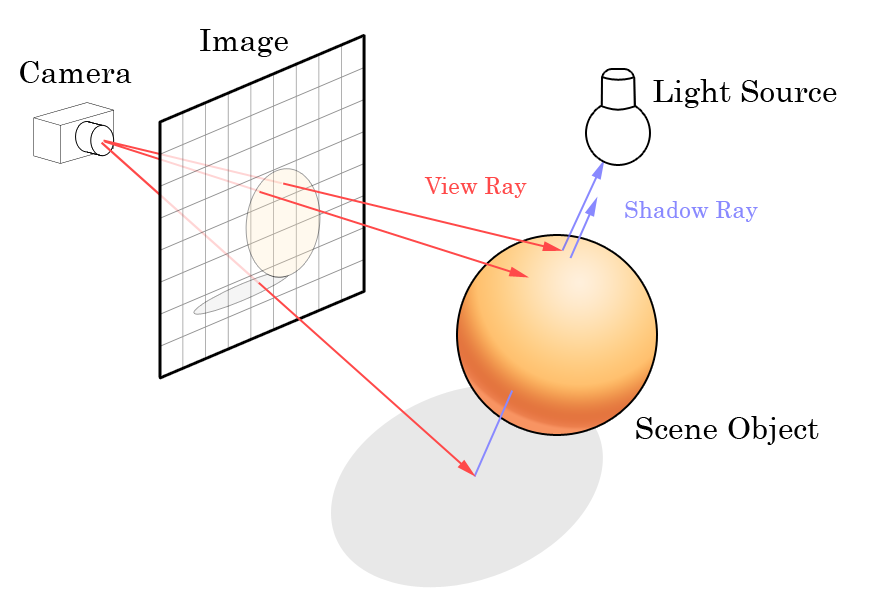
\includegraphics[width=.8\linewidth]{img/Ray_trace_diagram.png}
            \caption{Schéma représentant le lancer de rayons.}
            \label{img:opengl:raytracing}
        \end{figure}

        Cette technique de rendu est très populaire dans les applications de rendu différé, où l'on doit calculer non seulement la lumière donnée en un point, mais aussi les contributions des objets environnants à cette lumière. En effet, dans le monde réel, chaque corps noir émet de la lumière à une longueur d'onde déterminée par la quantité d'énergie qu'il possède. De plus, certains objets sont entièrement ou partiellement réflectifs, et propagent la lumière à d'autres endroits qui pourraient ne pas être éclairés directement.

        Le rendu par lancer de rayons possède beaucoup de qualités non négligeables pour le réalisme d'une scène, mais est malheureusement extrêmement coûteux à calculer. Certaines applications du lancer de rayons ne considèrent que la première interaction du rayon avec un objet de la scène, comme pour déterminer l'objet qu'un joueur pointe avec sa souris dans un jeu vidéo, par exemple. Notre technique de visualisation par sous-domaines utilise également cette technique, afin de déterminer le premier voxel contenant de l'information sur un rayon donné.

        Dû à la complexité associée au rendu par lancer de rayons, il fallut inventer une nouvelle façon de rendre un objet à l'écran : par rastérisation.
    }
    
    \subsubsection{Rastérisation}
    {
        Là où le lancer de rayons effectue une recherche depuis la caméra vers les objets, le processus de rastérisation effectue l'inverse. En effet, la technique de rendu par rastérisation utilise un ensemble de matrices afin de pouvoir projeter un objet 3D sur une matrice 2D (un écran, par exemple). En effet, il existe plusieurs façons de décrire la position d'un objet, selon le référentiel dans lequel on se place.
        
        En particulier, la rastérisation utilise principalement trois matrices :\begin{itemize}
            \item la matrice modèle ($\mathcal{M}$),
            \item la matrice de vue ($\mathcal{V}$),
            \item la matrice de projection ($\mathcal{P}$).
        \end{itemize}

        Ces trois matrices permettent de passer d'un système de coordonnées à un autre, afin de déterminer la position d'un point 3D dans un espace contenant la coordonnée 2D de l'objet, ainsi que sa profondeur par rapport au point de vue. Une fois cette transformation effectuée, les primitives géométriques sont projetées sur un plan 2D, pour générer un ensemble de fragments. Ces fragments sont le résutat d'une interpolation des coordonnées et propriétés d'un sommet d'une primitive en un point $P$, qui est la position d'un pixel dans ce plan 2D. Il suffit ensuite d'empiler les fragments en fonction de leur profondeur, prendre le premier fragment de chacune des piles comme celui à afficher et l'image est prête à être rendue à l'écran (voir figure \ref{img:opengl:raster}). Ce processus est non seulement beaucoup plus simple que le lancer de rayons, mais aussi beaucoup plus optimisée, car la complexité de cette méthode de rendu dépend principalement du nombre d'éléments à afficher à l'écran, au lieu de la complexité de la scène en elle-même.

        \begin{figure}
            \centering
            \begin{subfigure}{.48\linewidth}
                \centering
                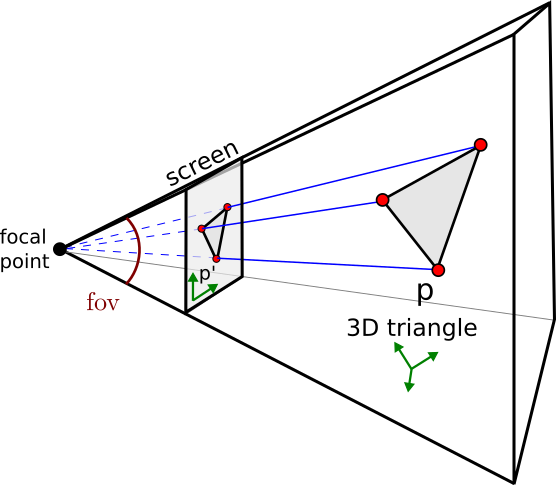
\includegraphics[width=.8\linewidth]{img/rasterization.png}
                \captionsetup{width=.8\linewidth}
                \caption{Projection du triangle sur un plan image 2D, avant la fragmentation.}
                \label{img:opengl:raster:projection}
            \end{subfigure}
            \begin{subfigure}{.48\linewidth}
                \centering
                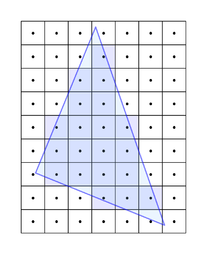
\includegraphics[width=.8\linewidth]{img/raster_to_frag.png}
                \captionsetup{width=.8\linewidth}
                \caption{Transformation depuis un triangle projeté à un ensemble de fragments.}
                \label{img:opengl:raster:fragments}
            \end{subfigure}
            \captionsetup{width=.6\linewidth}
            \caption{Le principe de rastérisation, en deux étapes.}
            \label{img:opengl:raster}
        \end{figure}

        Cette méthode de rendu est plus couramment utilisée dans des jeux vidéo, ou des applications de CAO, ou encore pour avoir une prévisualisation d'une scène que l'on va ensuite rendre au lancer de rayons, comme dans des logiciels tels que Blender par exemple.
    }
}

\subsection{OpenGL}
{
    OpenGL est une API\definition{Applicative Programming Interface} de rendu graphique multiplateforme. Cette API fut créée en 1992 par \textit{SiliconGraphics Inc.} afin de permettre d'accélérer la création de dessin 2D et 3D vectoriel sur un écran. Depuis 2006, OpenGL est maintenu par \textit{Khronos}, un consortium à but non-lucratif. \textit{Khronos} fournit OpenGL en tant que spécification technique, qui va ensuite être implémentée par des vendeurs tiers, tels que AMD, Nvidia, Intel (...). Cette spécification peut être implémentée de façon logicielle (comme le fait \textit{Mesa}\footnote{\url{https://www.mesa3d.org/}}), ou bien implémentée directement de façon matérielle, comme le font AMD ou Nvidia sur leurs cartes graphiques depuis quelques années. Dans ce cas là, l'API OpenGL est un ensemble d'appels systèmes qui effectuent directement des opérations complexes sur la carte graphique.
    
    OpenGL est spécifié comme une machine à états. Une fois que celle-ci est démarrée et activée, un contexte est créé et considéré comme valide pour utilisation par quiconque. L'utilisateur peut activer certaines fonctions, comme le test de profondeur ou encore l'utilisation de textures tridimensionnelles, et la machine interne à OpenGL mettra à jour son état afin de refléter au mieux l'état demandé par l'utilisateur. Ainsi, nous pouvons spécifier un état permettant d'utiliser les fonctionnalités nécessaires, envoyer un tableau de points et d'autres attributs à OpenGL afin d'afficher à l'écran l'ensemble de points demandés. Lorsque OpenGL rentre dans l'état de rendu, il effectue un processus de traitement des données en entrée afin de pouvoir afficher une primitive à l'écran. Cet état de rendu possède deux méthodes de calcul : le mode direct, et le mode indirect.

    \paragraph{Mode direct}
    {
        Durant un rendu en mode direct, OpenGL ne prend en entrée que les points spécifiés par l'utilisateur à ce moment donné. Il effectue son traitements de points dessus, et affiche le résultat à l'écran, ou sur une surface quelconque. Dans ce mode, OpenGL ne retient en aucun cas les informations passées par l'utilisateur, et n'affiche qu'une seule fois le résultat des opérations sur les points. Ce mode est souvent utilisé pour faire un affichage d'un point à l'écran à des fins de débogage, bien qu'il soit déprécié dans les versions d'OpenGL courantes (4.6 actuellement).
    }

    \paragraph{Mode indirect}
    {
        Durant un rendu en mode indirect, OpenGL va aller chercher les points à rendre à l'écran dans des tableaux alloués sur demande de l'utilisateur dans l'espace mémoire alloué à OpenGL, que ce soit en mémoire RAM ou en mémoire vidéo, sur une carte graphique par exemple. Ainsi, afin de rendre un objet à l'écran en mode indirect, il est nécessaire de l'allouer et de spécifier à OpenGL la disposition mémoire nécessaire pour différencier les positions des normales, des couleurs (...) et ainsi de suite.

        Ce mode indirect permet aussi de personnaliser le processus de traitement des données, grâce à l'utilisation de \textit{shaders}. En effet, même si les opérations qu'effectue OpenGL afin d'afficher un élément à l'écran ne sont pas interchangeables, elles sont pour la plupart programmables. Ainsi, tout au long du processus de traitement des données (détaillé en figure \ref{img:opengl:rendering_pipeline}), il est possible de programmer les étapes telles que le traitement des sommets, le traitement des pixels après rastérisation, ou encore l'assemblage géométrique des points en primitives.

        \begin{figure}[h]
            \centering
            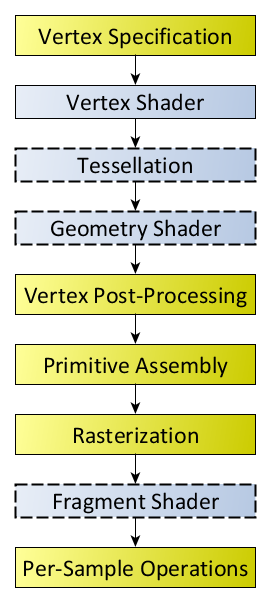
\includegraphics[width=.2\linewidth]{img/RenderingPipeline.png}
            \caption{Traitement des primitives par OpenGL. Les étapes dont le bord est en pointillé sont programmables.}
            \label{img:opengl:rendering_pipeline}
        \end{figure}
    }

    Ainsi, nous avons pu voir les deux modes principaux qu'utilise OpenGL afin d'afficher une primitive à l'écran. Le mode direct est rapide, mais ne retient pas les actions de l'utilisateur pour l'affichage au temps $t~+~\delta_t$. Le mode indirect est efficace, et permet de garder en mémoire les opérations à effectuer, et permet d'utiliser des accélérateurs de calcul externes, tels que des cartes graphiques.
}